\chapter{Useful Python}

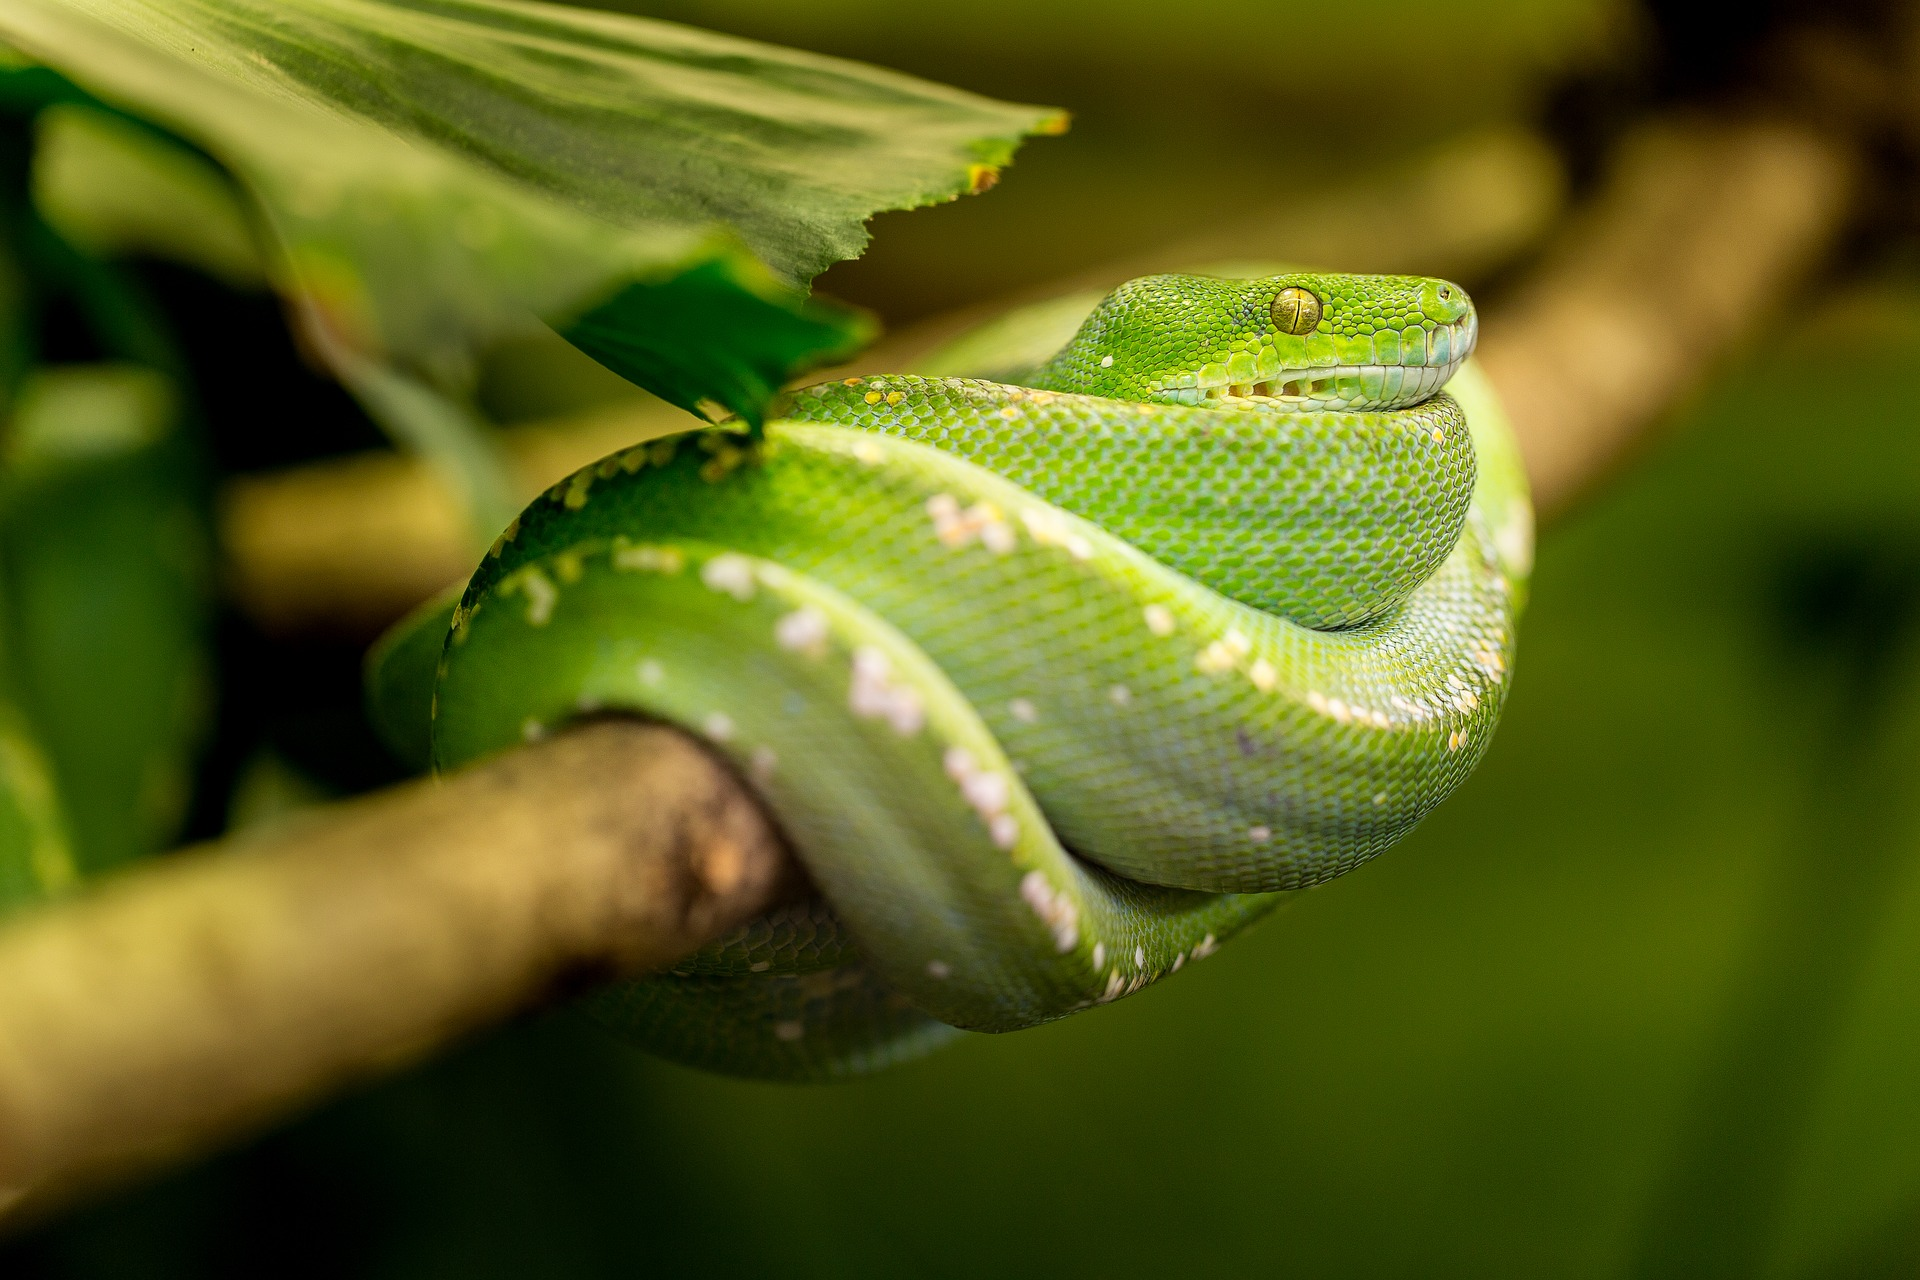
\includegraphics{24-python.jpg}

\justifying
Getting started in writing programs is easy with Python. It is a highly extensible language with many add on modules available.
There is a collection known as Pypi where many of these Open Source\index{OpenSource} modules are hosted.
Python is fairly easy to learn, especially when compared to other languages. Python runs ``everywhere'', for all intents and
purposes. With it's gentle learning vurve, it has become the go to language for Data Scientists, System Administrators, and yes, even
DevSecOps folks like ourselves. For all these reasons, Python makes a great addition to our toolbox.

\justifying
An item of note, Python3 is our only choice at this point. Python 2.x End of Life was January 1st, 2020.

\section{Local Development Environment}

\markdownInput{../labs/24-python/lab-24-python-a.md}

\section{Project Layout}

\subsection{Python Directory Structure}
\justifying
Files and folders relevant to the Python portions of our project are shown in the diagram below.

\begin{figure}[!htb]
	\centering
	\chapter{Useful Python}

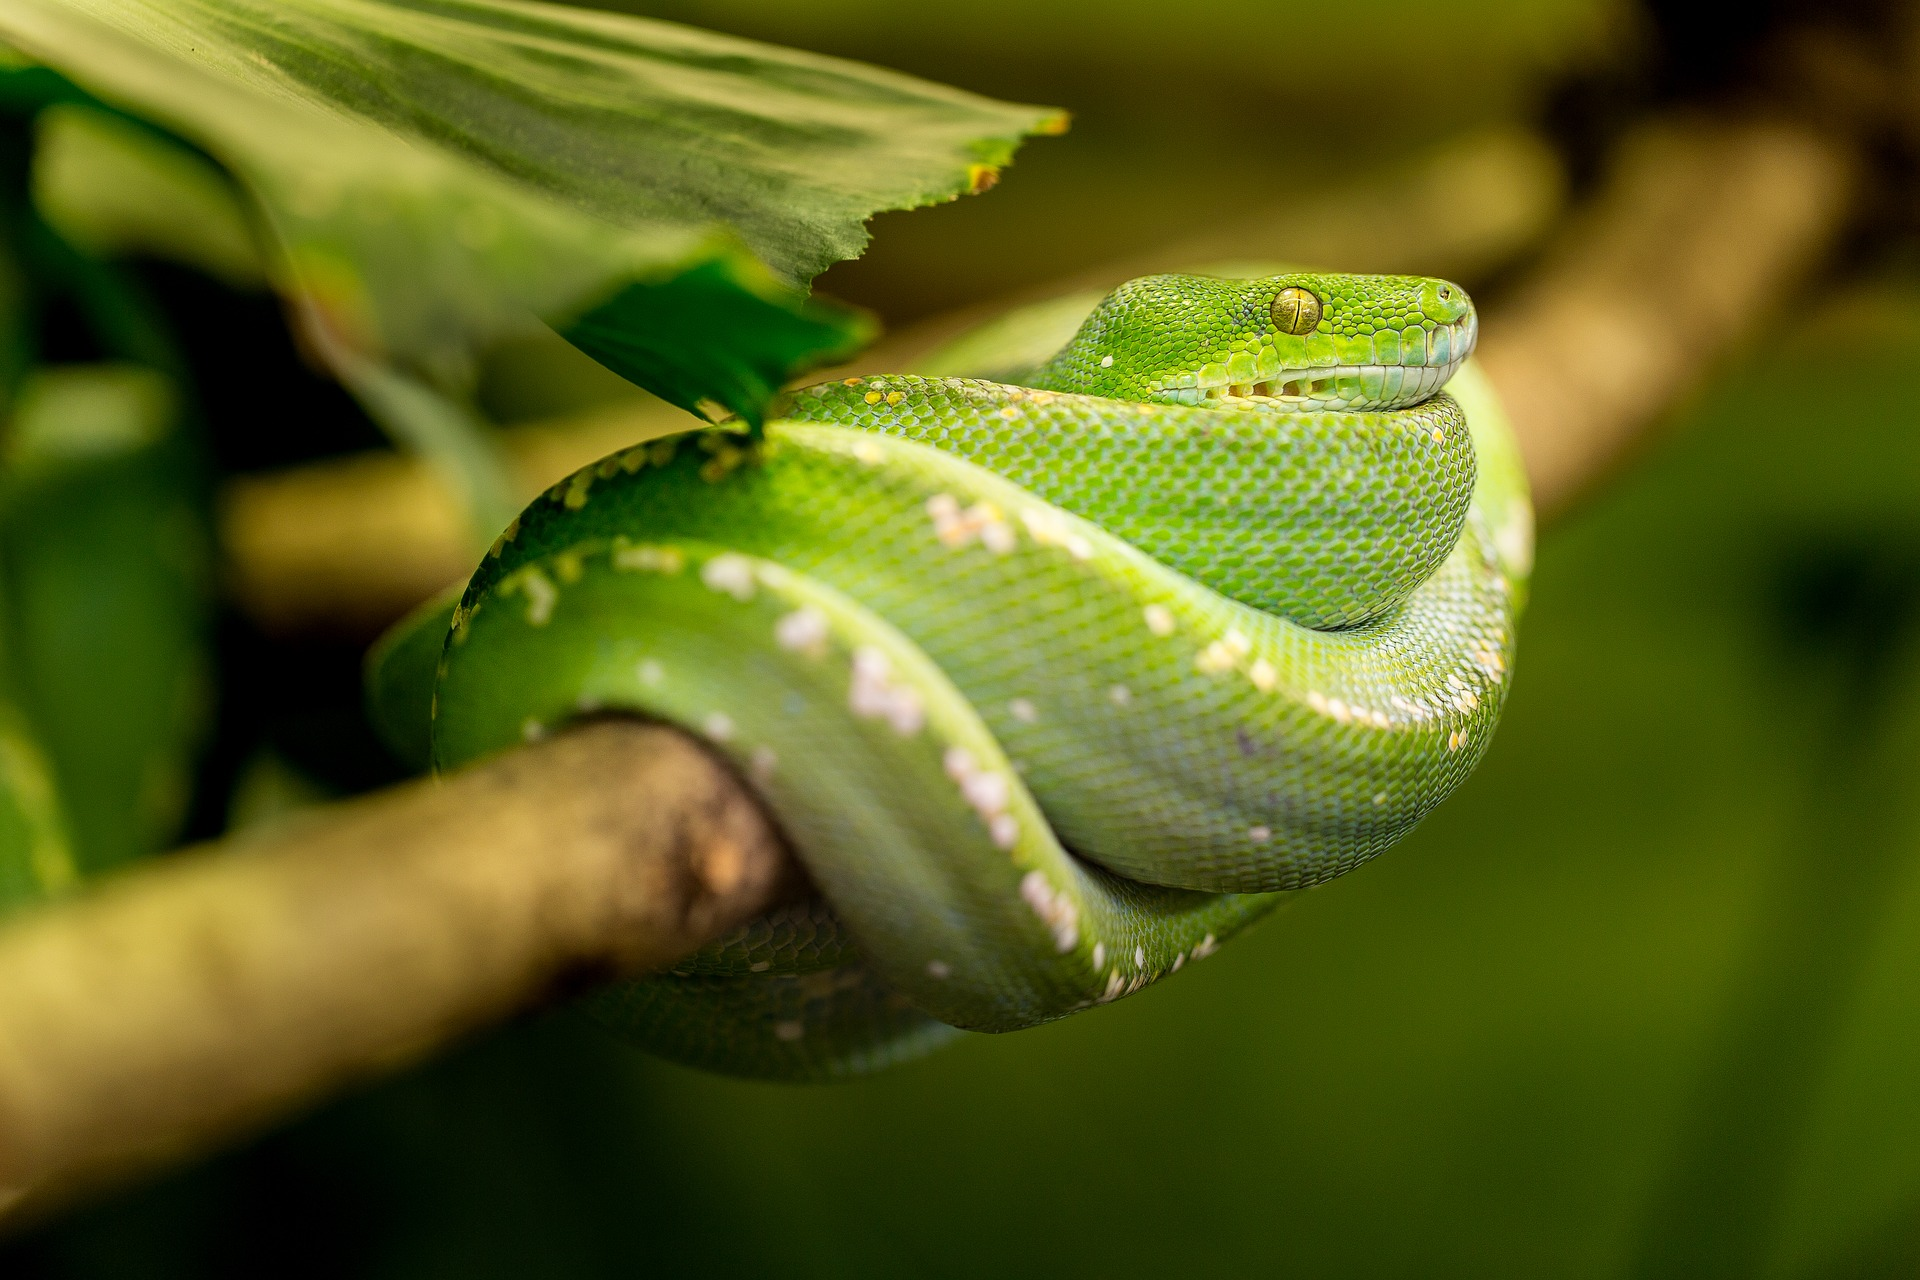
\includegraphics{24-python.jpg}

\justifying
The Python language is good for newcomers and experienced practitioners alike. Python is a highly extensible language with many add on modules available.
There is a collection known as \href{https://pypi.org/}{Pypi} where many of these Open Source\index{OpenSource} module projects are hosted. Python has a
fairly gentle learning curve, especially when compared to other languages. Python runs ``everywhere'', for all intents and purposes. With it's gentle
learning curve, it has become the go to language for Data Scientists, System Administrators, and yes, even DevSecOps folks like ourselves. For all these
reasons, Python makes a great addition to our toolbox.

\justifying
The goal of this chapter is not to teach you how to program with Python. There are many existing, well written resources already available on the Internet
that can help you with this. Our purpose here is derive repeatable patterns and best practices that can help us realize reusability and scalability in our projects. In other words, we will focus on some things that will get your projects up and running quickly.

\justifying
Consistently putting our files in the same places with the same naming convention becomes helpful as the number of projects we accumulate over the years
grows from the tens into the hundreds. This strategy can also help with code reuse across projects, as bits of codes can be quickly copied to new projects
or used to refresh existing projects with minimal refactoring.

\justifying
An item of note, Python3 is our only choice at this point. Python 2.x End of Life was January 1st, 2020.

\section{Local Development Environment}

\justifying
Support for modern operating systems is available, and installation of the necessary files to support Python is a relatively painless experience.

\markdownInput{../labs/24-python/lab-24-python-a.md}

\section{Python Virtual Environments}

\justifying
Temporary virtual environments allow us to confine the dependencies for our project to a temporary workspace.
This is preferable to installing project dependencies directly to a development workstation, as we may be
testing with modules that could corrupt the working configuration on the workstation.

\markdownInput{../labs/24-python/lab-24-python-b.md}

\section{Requirements Files}

\justifying
A requirements file lists the required Python modules needed to build and run any Python portions of our
project. We also add a check in the Makefile to verify the existence of the requirements.txt file.

\justifying
Some requirements are strictly intended to be part of the test harness, but are not needed for the application
proper. Using a separate file, such as tests/requirements-test.txt, makes this delineation clear to folks who are not familiar with the project.

\markdownInput{../labs/24-python/lab-24-python-c.md}

\section{The \_\_init\_\_.py File}

\justifying
We add this file to let the Python interpreter know that the directories the file is found in are a contiguous part of our Python project. Since module
imports and function definitions in this file are available to all the Python code files in the directory, we can use it to our advantage. For example, try
adding this quick and dirty logging function to src/\_\_init\_\_.py

\justifying
\begin{mybox}{\thetcbcounter: \_\_init\_\_.py}
  \lstinputlisting{code/24-python/init.py}
\end{mybox}

\section{Logging Framework}
\justifying
Now we can create a Python file ``src/logging.py'' and call the logger from within like so:

\begin{mybox}{\thetcbcounter: logging.py}
    \lstinputlisting{code/24-python/logtest.py}
\end{mybox}

\justifying
Check the results in the file /var/log/devsecops/devsecops.log.

\section{Logging Framework}

\justifying
We can create a file to define the characteristics of our logging mechanism.

\begin{mybox}{\thetcbcounter: logging.conf}
	\lstinputlisting{code/24-python/logging.conf}
\end{mybox}

\justifying
Now we can use this framework in the source files for our project.

\begin{mybox}{\thetcbcounter: logging}
	\lstinputlisting{code/24-python/logging-config}
\end{mybox}

\section{Python Directory Structure}
\justifying
Files and folders relevant to the Python portions of our project are shown in the diagram below.

\begin{figure}[!htb]
	\centering
	\chapter{Useful Python}

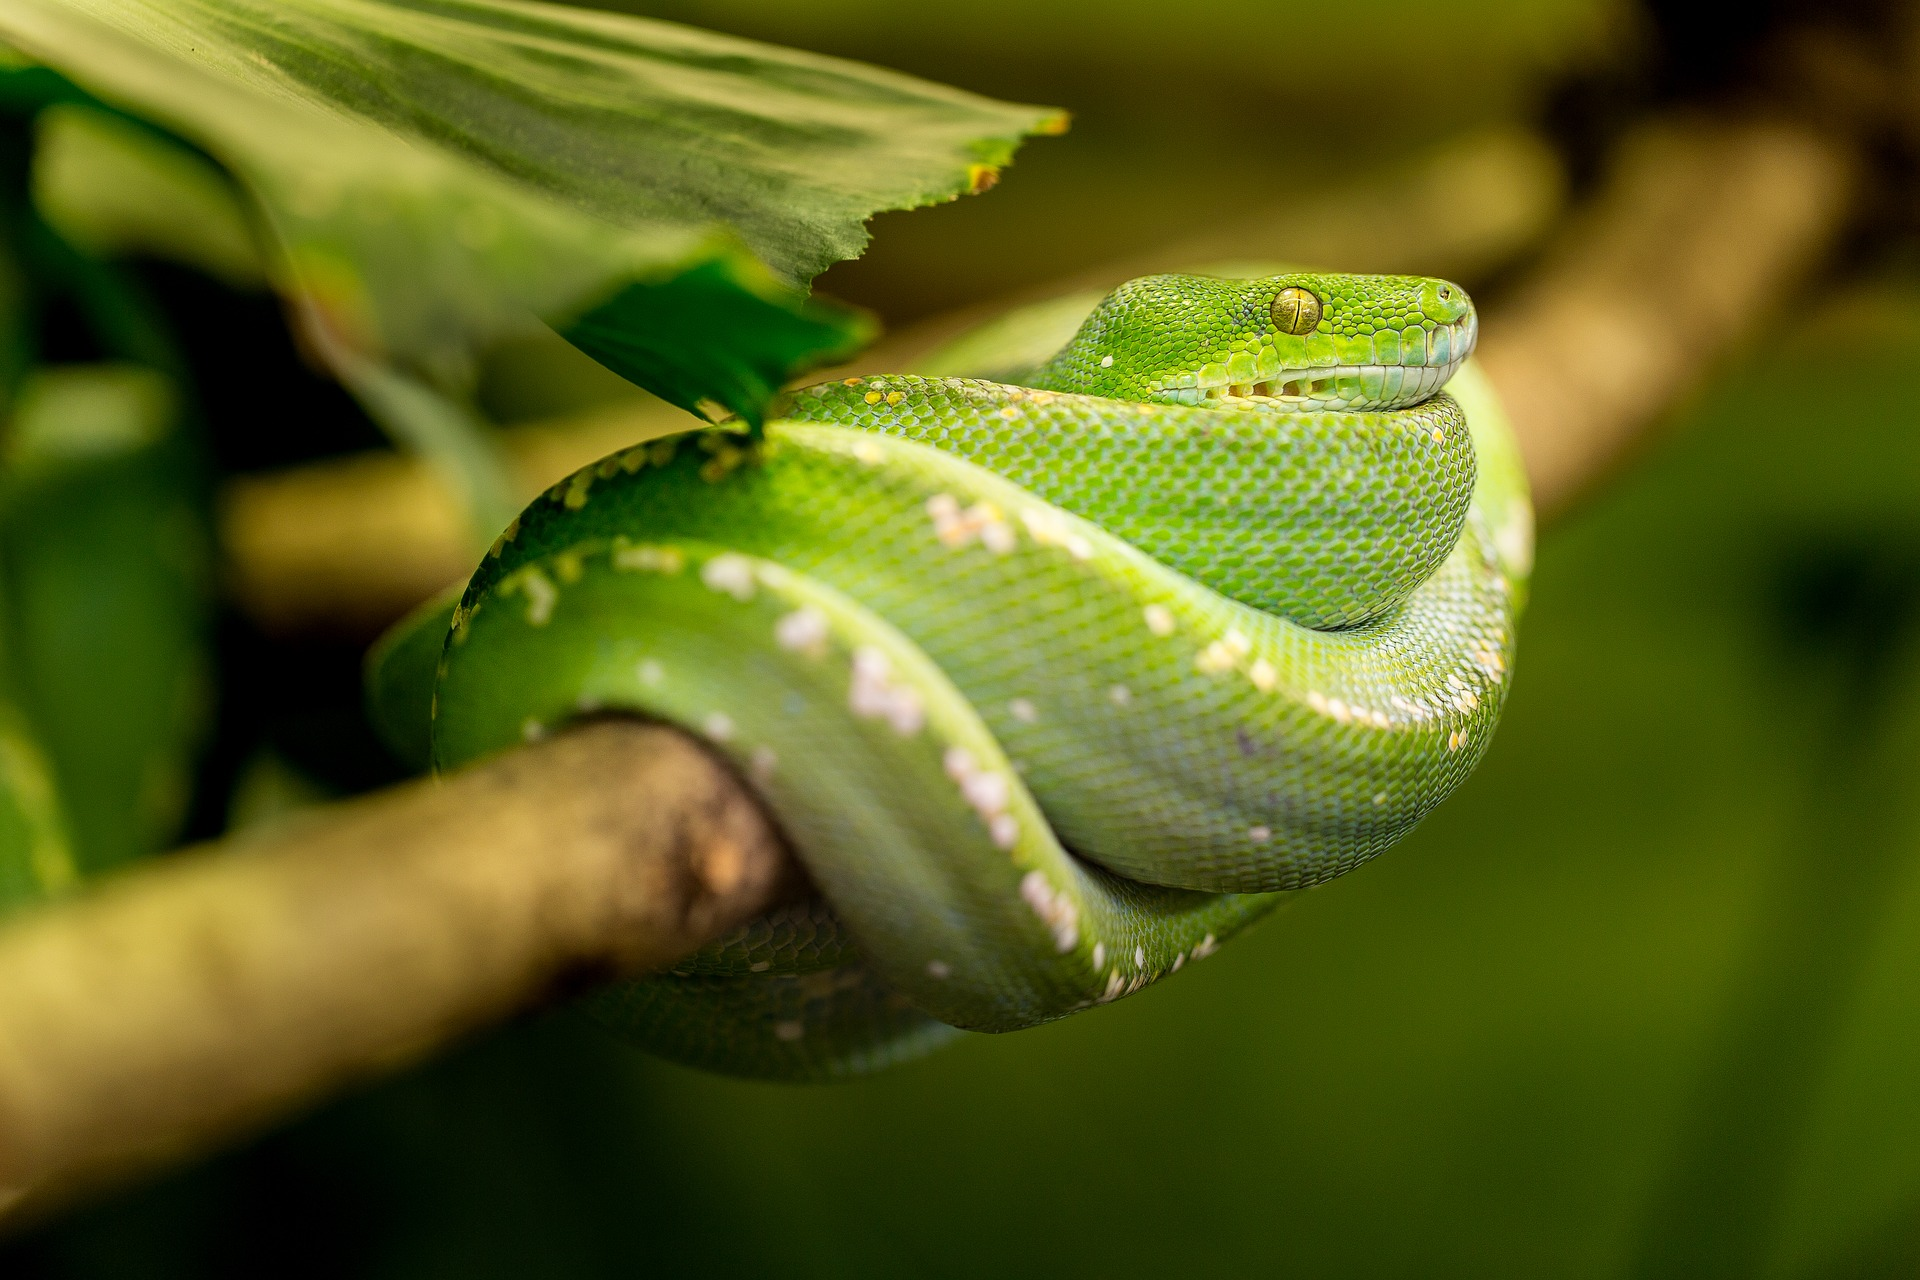
\includegraphics{24-python.jpg}

\justifying
The Python language is good for newcomers and experienced practitioners alike. Python is a highly extensible language with many add on modules available.
There is a collection known as \href{https://pypi.org/}{Pypi} where many of these Open Source\index{OpenSource} module projects are hosted. Python has a
fairly gentle learning curve, especially when compared to other languages. Python runs ``everywhere'', for all intents and purposes. With it's gentle
learning curve, it has become the go to language for Data Scientists, System Administrators, and yes, even DevSecOps folks like ourselves. For all these
reasons, Python makes a great addition to our toolbox.

\justifying
The goal of this chapter is not to teach you how to program with Python. There are many existing, well written resources already available on the Internet
that can help you with this. Our purpose here is derive repeatable patterns and best practices that can help us realize reusability and scalability in our projects. In other words, we will focus on some things that will get your projects up and running quickly.

\justifying
Consistently putting our files in the same places with the same naming convention becomes helpful as the number of projects we accumulate over the years
grows from the tens into the hundreds. This strategy can also help with code reuse across projects, as bits of codes can be quickly copied to new projects
or used to refresh existing projects with minimal refactoring.

\justifying
An item of note, Python3 is our only choice at this point. Python 2.x End of Life was January 1st, 2020.

\section{Local Development Environment}

\justifying
Support for modern operating systems is available, and installation of the necessary files to support Python is a relatively painless experience.

\markdownInput{../labs/24-python/lab-24-python-a.md}

\section{Python Virtual Environments}

\justifying
Temporary virtual environments allow us to confine the dependencies for our project to a temporary workspace.
This is preferable to installing project dependencies directly to a development workstation, as we may be
testing with modules that could corrupt the working configuration on the workstation.

\markdownInput{../labs/24-python/lab-24-python-b.md}

\section{Requirements Files}

\justifying
A requirements file lists the required Python modules needed to build and run any Python portions of our
project. We also add a check in the Makefile to verify the existence of the requirements.txt file.

\justifying
Some requirements are strictly intended to be part of the test harness, but are not needed for the application
proper. Using a separate file, such as tests/requirements-test.txt, makes this delineation clear to folks who are not familiar with the project.

\markdownInput{../labs/24-python/lab-24-python-c.md}

\section{The \_\_init\_\_.py File}

\justifying
We add this file to let the Python interpreter know that the directories the file is found in are a contiguous part of our Python project. Since module
imports and function definitions in this file are available to all the Python code files in the directory, we can use it to our advantage. For example, try
adding this quick and dirty logging function to src/\_\_init\_\_.py

\justifying
\begin{mybox}{\thetcbcounter: \_\_init\_\_.py}
  \lstinputlisting{code/24-python/init.py}
\end{mybox}

\section{Logging Framework}
\justifying
Now we can create a Python file ``src/logging.py'' and call the logger from within like so:

\begin{mybox}{\thetcbcounter: logging.py}
    \lstinputlisting{code/24-python/logtest.py}
\end{mybox}

\justifying
Check the results in the file /var/log/devsecops/devsecops.log.

\section{Logging Framework}

\justifying
We can create a file to define the characteristics of our logging mechanism.

\begin{mybox}{\thetcbcounter: logging.conf}
	\lstinputlisting{code/24-python/logging.conf}
\end{mybox}

\justifying
Now we can use this framework in the source files for our project.

\begin{mybox}{\thetcbcounter: logging}
	\lstinputlisting{code/24-python/logging-config}
\end{mybox}

\section{Python Directory Structure}
\justifying
Files and folders relevant to the Python portions of our project are shown in the diagram below.

\begin{figure}[!htb]
	\centering
	\chapter{Useful Python}

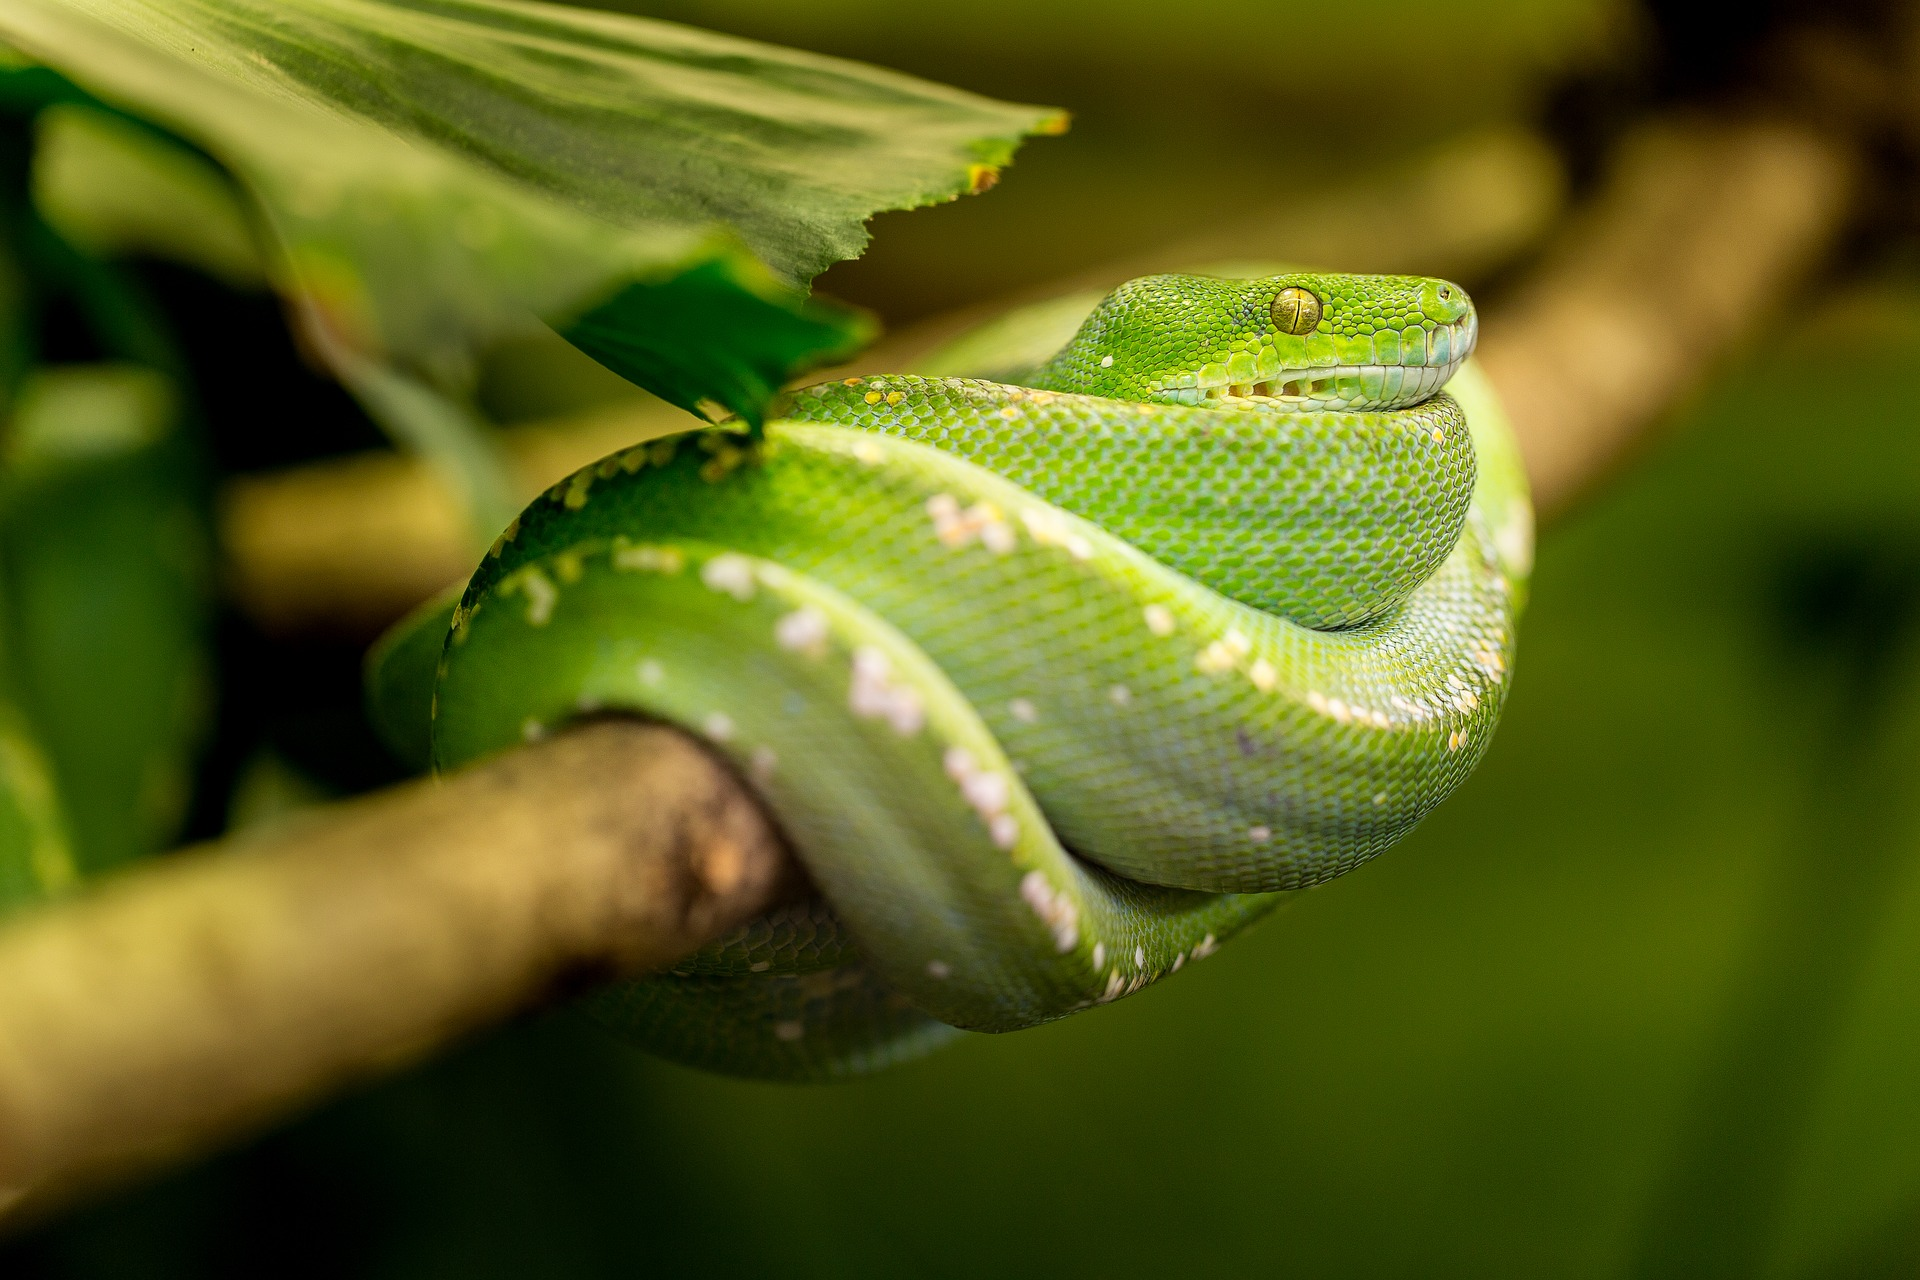
\includegraphics{24-python.jpg}

\justifying
The Python language is good for newcomers and experienced practitioners alike. Python is a highly extensible language with many add on modules available.
There is a collection known as \href{https://pypi.org/}{Pypi} where many of these Open Source\index{OpenSource} module projects are hosted. Python has a
fairly gentle learning curve, especially when compared to other languages. Python runs ``everywhere'', for all intents and purposes. With it's gentle
learning curve, it has become the go to language for Data Scientists, System Administrators, and yes, even DevSecOps folks like ourselves. For all these
reasons, Python makes a great addition to our toolbox.

\justifying
The goal of this chapter is not to teach you how to program with Python. There are many existing, well written resources already available on the Internet
that can help you with this. Our purpose here is derive repeatable patterns and best practices that can help us realize reusability and scalability in our projects. In other words, we will focus on some things that will get your projects up and running quickly.

\justifying
Consistently putting our files in the same places with the same naming convention becomes helpful as the number of projects we accumulate over the years
grows from the tens into the hundreds. This strategy can also help with code reuse across projects, as bits of codes can be quickly copied to new projects
or used to refresh existing projects with minimal refactoring.

\justifying
An item of note, Python3 is our only choice at this point. Python 2.x End of Life was January 1st, 2020.

\section{Local Development Environment}

\justifying
Support for modern operating systems is available, and installation of the necessary files to support Python is a relatively painless experience.

\markdownInput{../labs/24-python/lab-24-python-a.md}

\section{Python Virtual Environments}

\justifying
Temporary virtual environments allow us to confine the dependencies for our project to a temporary workspace.
This is preferable to installing project dependencies directly to a development workstation, as we may be
testing with modules that could corrupt the working configuration on the workstation.

\markdownInput{../labs/24-python/lab-24-python-b.md}

\section{Requirements Files}

\justifying
A requirements file lists the required Python modules needed to build and run any Python portions of our
project. We also add a check in the Makefile to verify the existence of the requirements.txt file.

\justifying
Some requirements are strictly intended to be part of the test harness, but are not needed for the application
proper. Using a separate file, such as tests/requirements-test.txt, makes this delineation clear to folks who are not familiar with the project.

\markdownInput{../labs/24-python/lab-24-python-c.md}

\section{The \_\_init\_\_.py File}

\justifying
We add this file to let the Python interpreter know that the directories the file is found in are a contiguous part of our Python project. Since module
imports and function definitions in this file are available to all the Python code files in the directory, we can use it to our advantage. For example, try
adding this quick and dirty logging function to src/\_\_init\_\_.py

\justifying
\begin{mybox}{\thetcbcounter: \_\_init\_\_.py}
  \lstinputlisting{code/24-python/init.py}
\end{mybox}

\section{Logging Framework}
\justifying
Now we can create a Python file ``src/logging.py'' and call the logger from within like so:

\begin{mybox}{\thetcbcounter: logging.py}
    \lstinputlisting{code/24-python/logtest.py}
\end{mybox}

\justifying
Check the results in the file /var/log/devsecops/devsecops.log.

\section{Logging Framework}

\justifying
We can create a file to define the characteristics of our logging mechanism.

\begin{mybox}{\thetcbcounter: logging.conf}
	\lstinputlisting{code/24-python/logging.conf}
\end{mybox}

\justifying
Now we can use this framework in the source files for our project.

\begin{mybox}{\thetcbcounter: logging}
	\lstinputlisting{code/24-python/logging-config}
\end{mybox}

\section{Python Directory Structure}
\justifying
Files and folders relevant to the Python portions of our project are shown in the diagram below.

\begin{figure}[!htb]
	\centering
	\input{dot/24-python.tex}
	\caption{Project directory and related files.}
	\label{pythonfiles}
\end{figure}

	\caption{Project directory and related files.}
	\label{pythonfiles}
\end{figure}

	\caption{Project directory and related files.}
	\label{pythonfiles}
\end{figure}

	\caption{Project directory and related files.}
	\label{pythonfiles}
\end{figure}

\subsection{The \_\_init\_\_.py File}

\justifying
We add this file to let the Python interpreter know that the directories
it is found in are a contiguous part of our Python project. Since module
imports and function definitions in this file are available to all the
python code files in the directory, we can use it to our advantage. For
example, try adding this quick and dirty logging function to
python/devsecops/lib/\_\_init\_\_.py

\justifying
\begin{mybox}{\thetcbcounter: \_\_init\_\_.py}
  \lstinputlisting{code/24-python/init.py}
\end{mybox}

\justifying
Now we can create a Python file log\_test.py and call the logger from within like so:

\begin{mybox}{\thetcbcounter: logtest.py}
  \lstinputlisting{code/24-python/logtest.py}
\end{mybox}

\justifying
Check the results in the file /var/log/devsecops/devsecops.log.

\subsection{Requirements File}

\justifying
A requirements file under python/requirements.txt\index{requirements.txt} lists
the required Python modules needed to build and run any Python portions of our  project.
We also add a check in the Makefile to verify the existence of the requirements.txt file.
The intention is, so we can quickly cut and paste the Makefile into a new project, but
not break anything if no requirements are present yet.

\subsection{Logging Framework}

\section{Python Virtual Environments}

\section{Python Testing}

\justifying
Security and reliability in our lab and rapid prototyping work is just as important as it is in our work for the Production environment.
In fact, you might say it's even more important since today's rapid mock ups
can easily wind up making it into the build pipeline when folks are under a time crunch to deliver.

\justifying
There are many test frameworks out there, lots of great ideas put forth by the community. For our current
efforts, we've settled on Tox\index{Tox} as the framework of choice. It dovetails nicely with the rest of
our patterns. Tox allows us to manage requirements for virtual environments when testing, acts as a front
end to pytest and coverage modules, and much more. It is highly configurable and extensible. For example
we can test that an application is compatible with multiple versions of Python.

\justifying
Use the make test command inside the docker container to run the test suite for the project.

\justifying
An example tox.ini\index{tox.ini} file follows. Take notice of the ``deps'' section,
where Python module requirements can be specified. In our current configuration,
these are in lieu of test harness requirements specified in our
python/requirements-test.txt file.

\begin{mybox}{\thetcbcounter: An example tox.ini file}
	\lstinputlisting{code/24-python/tox.ini}
\end{mybox}

\justifying
Note that we can also include test requirements outside of our tox.ini file, as detailed in the next section.

\subsection{Python Test Requirements}

\justifying
Some requirements are strictly intended to be part of the test harness, but are not
needed for the application proper. Using a separate file, such as
python/requirements-test.txt, makes this delineation clear to folks who are not familiar with the project.

\subsection{Unit Test Cases}

\justifying
Unit and functional testing is foundational in developing robust, secure
code. We want to be sure that when we create new code, we are also adding
test cases to our test suite that fully cover the new classes, functions, and so on.

\justifying
Consider the following example unit test case. The purpose is to test
that the function check\_docker() in the file python/devsecops/lib/helper\_functions.py
returns True when called from inside a Docker container.

\begin{mybox}{\thetcbcounter: An example Unit test case}
  \lstinputlisting{code/24-python/test-unit-example.py}
\end{mybox}

\subsection{Test Coverage}

\justifying
As mentioned previously, we can avail ourselves of the coverage module by adding it to test-requirements.txt or
the deps section of our tox.ini file. The purpose is to automatically generate a report on how much of our code
is ``covered'' by test cases in python/test.

\subsection{Linting with Tox}

Recall that we are using Tox as our main test framework. To set up Tox
to do our linting work for us, we can add an environment to our envlist
called ``pylint'' and then declare it in a new stanza in tox.ini. Notice
how we let ``deps'' do the work of installing the ``pylint'' dependency for
us.

\begin{mybox}{\thetcbcounter: An Example tox.ini file}
    \lstinputlisting{code/41-cicd/toxfile-pylint}
\end{mybox}
